\section{Use Cases}

\subsection{Actors}
An actor specifies a role that are to be played by an external person interacting with our application. We have only one actor, and that is the regular user:  A person who don’t have much education in using our app, but who will use it regularly in his workday.

\subsection{Use case diagrams}
See figure \ref{fig:usecase} at page \pageref{fig:usecase}.

\begin{figure}
\begin{center}
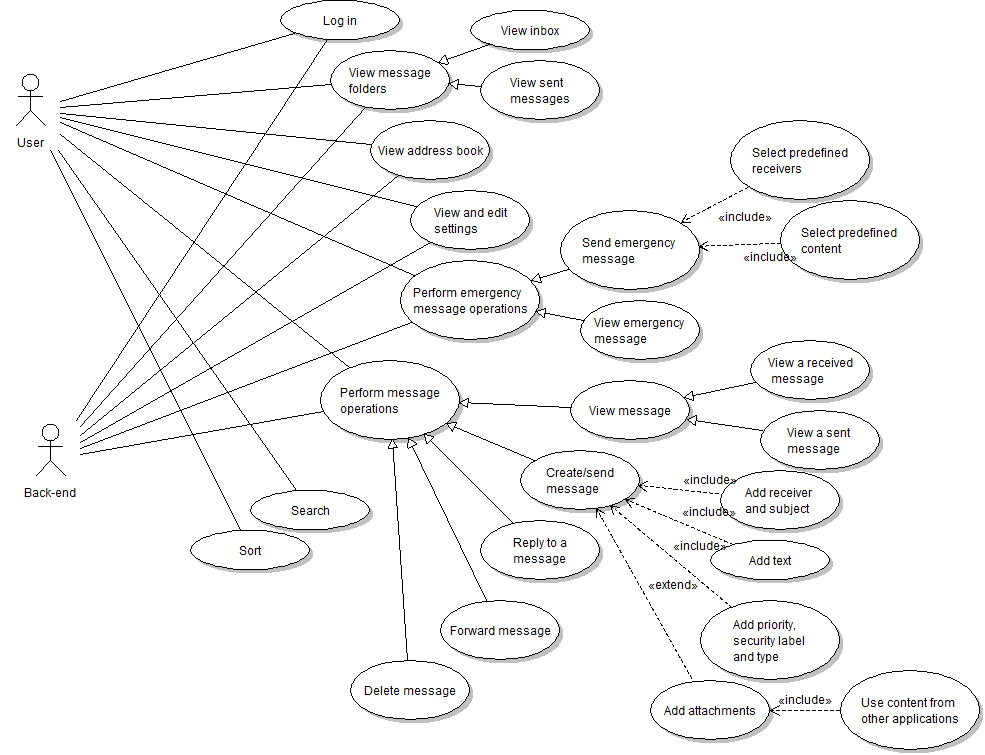
\includegraphics[width=\textwidth]{kpro-use-case}
\caption{Use case diagram} \label{fig:usecase}
\end{center}
\end{figure}

\subsection{Textual use cases}
Each of the use cases is described below, so that the use case diagram will be easier to understand. See table \ref{tab:viewmessages} - \ref{tab:settings} starting at page \pageref{tab:viewmessages} for a more detailed explanation of the use cases.


\begin{table}
\begin{tabular}{p{3cm}p{12cm}}
& 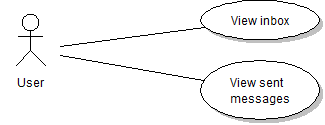
\includegraphics{view_messages}\\ \hline
Element & Description \\ \hline
Use case name & View messages \\
Goal & View received and sent messages \\
Summary &The user would like to view received and sent messages \\
Preconditions &
\begin{enumerate}
\item{}The application is running.
\item{}The user is logged in.
\end{enumerate} \\ \hline
Flow of Events &
\begin{enumerate}
\item{}The user selects a message from either the inbox or sent messages.
\item{}Message is showed to user.
\end{enumerate} \\ \hline
Exceptions & There are no existing messages.
\end{tabular}
\caption{View messages textual use case} \label{tab:viewmessages}
\end{table}

\begin{table}
\begin{tabular}{p{3cm}p{12cm}}
& 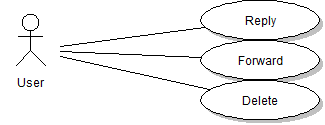
\includegraphics{reply_forward_delete}\\ \hline
Element & Description \\ \hline
Use case name & Reply, forward and delete \\
Goal & Reply, forward and delete messages\\
Summary & The user would like to reply to a message, forward it or delete it. \\
Preconditions &
\begin{enumerate}
\item{}The application is running.
\item{}The user is logged in.
\end{enumerate} \\ \hline
Flow of Events &
\begin{enumerate}
\item{}The user selects a message from either the sent or inbox messages.
\item{}Message is showed to user.
\item{}User chooses to reply, forward or delete the message. 
\end{enumerate} \\ \hline
Exceptions & There are no existing messages.
\end{tabular}
\caption{Reply, forward and delete textual use case} \label{tab:viewmessages}
\end{table}

\begin{table}
\begin{tabular}{p{3cm}p{12cm}}
& 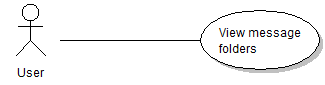
\includegraphics{view_message_folders}\\ \hline
Element & Description \\ \hline
Use case name & View message folders \\
Goal & View inbox and sent messages \\
Summary &The user would like to view the inbox and a list of sent messages \\
Preconditions &
\begin{enumerate}
\item{}The application is running.
\item{}The user is logged in.
\end{enumerate} \\ \hline
Flow of Events &
\begin{enumerate}
\item{}The user enters the inbox or sent messages.
\item{}The list of messages in the inbox or sent messages is presented to the user.
\end{enumerate} \\ \hline
Exceptions & There are no existing messages.
\end{tabular}
\caption{View message folders use case} \label{tab:viewmessages}
\end{table}

\begin{table}
\begin{tabular}{p{3cm}p{12cm}}
& 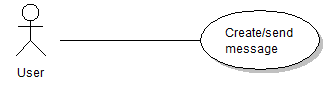
\includegraphics{create_message}\\ \hline
Element & Description \\ \hline
Use case name & Create message \\
Goal & User creates and sends a complete message \\
Summary &The user would like to create/send a message to a receiver with a subject and text. The user would also like to set the priority, security label and type of the message as well as being able to add an attachment from other applications. \\
Preconditions &
\begin{enumerate}
\item{}The application is running.
\item{}The user is logged in.
\end{enumerate} \\ \hline
Flow of Events &
\begin{enumerate}
\item{}User selects new message.
\item{}The user adds the recipient(s) and subject to the message.
\item{}The user sets the priority, security label and type.
\item{}The user adds attachments if needed.
\end{enumerate} \\ \hline
Exceptions & The user does not set priority, security label and type and default values are set.
\end{tabular}
\caption{Create message textual use case} \label{tab:createmessage}
\end{table}

\begin{table}
\begin{tabular}{p{3cm}p{12cm}}
& 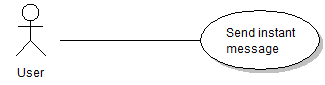
\includegraphics{send_instant_message}\\ \hline
Element & Description \\ \hline
Use case name & Send instant message \\
Goal & User sends an instant message \\
Summary & The user sends an instant message with predefined content to predefined receivers \\
Preconditions &
\begin{enumerate}
\item{}The application is running.
\item{}The user is logged in.
\end{enumerate} \\ \hline
Flow of Events &
\begin{enumerate}
\item{}User selects new instant message.
\item{}The user sends the message.
\end{enumerate} \\ \hline
Exceptions & The predefined values have not been set.
\end{tabular}
\caption{Send instant message textual use case} \label{tab:createmessage}
\end{table}

\begin{table}
\begin{tabular}{p{3cm}p{12cm}}
& 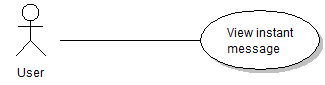
\includegraphics{view_instant_message}\\ \hline
Element & Description \\ \hline
Use case name & View instant message \\
Goal & User views an instant message \\
Summary & The user receives and viesw an instant message \\
Preconditions &
\begin{enumerate}
\item{}The application is running.
\item{}The user is logged in.
\end{enumerate} \\ \hline
Flow of Events &
\begin{enumerate}
\item{}User receives an instant message.
\item{}A popup appear on the users screen.
\item{}User presses the popup and views the instant message.
\end{enumerate} \\ \hline
\end{tabular}
\caption{View instant message textual use case} \label{tab:createmessage}
\end{table}

\begin{table}
\begin{tabular}{p{3cm}p{12cm}}
& 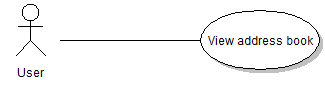
\includegraphics{view_address_book}\\ \hline
Element & Description \\ \hline
Use case name & View and interact with address book \\
Goal & User can view and interact with the address book \\
Summary &The user enters the address book and is able to view, add, edit and delete contacts. \\
Preconditions &
\begin{enumerate}
\item{}The application is running.
\item{}The user is logged in.
\end{enumerate} \\ \hline
Flow of Events &
\begin{enumerate}
\item{}User selects address book.
\item{}User either adds a new contact or selects an existing one.
\item{}If the user selects an existing contact, he can either edit that contact or delete it.
\end{enumerate}
\end{tabular}
\caption{View and interact textual use case} \label{tab:viewandinteract}
\end{table}

\begin{table}
\begin{tabular}{p{3cm}p{12cm}}
& 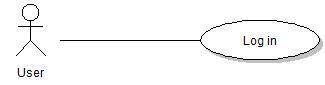
\includegraphics{login}\\ \hline
Element & Description \\ \hline
Use case name & Log in \\
Goal & User logs in with a username and password. \\
Summary &The user is prompted with a login screen and must type in his username and password. \\
Preconditions &
\begin{enumerate}
\item{}The application is running.
\end{enumerate} \\ \hline
Flow of Events &
\begin{enumerate}
\item{}User starts application.
\item{}User is prompted with username and password.
\item{}User types in username and password and presses the login button.
\item{}User gains access to the application data and functionality.
\end{enumerate} \\ \hline
Exceptions & User types wrong username and password and is denied access.
\end{tabular}
\caption{Log in textual use case} \label{tab:login}
\end{table}

\begin{table}
\begin{tabular}{p{3cm}p{12cm}}
& 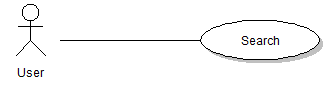
\includegraphics{search}\\ \hline
Element & Description \\ \hline
Use case name & Search \\
Goal & User receives search results for a given search text. \\
Summary & The user search in the application for mail, contacts etc through a search field at the top of the screen. \\
Preconditions &
\begin{enumerate}
\item{}The application is running.
\item{}The user is logged in.
\end{enumerate} \\ \hline
Flow of Events &
\begin{enumerate}
\item{}User highlights search field and inserts his the text he wants to search for.
\item{}User presses the search button.
\item{}Application shows search results to the user.
\end{enumerate}
\end{tabular}
\caption{Search textual use case} \label{tab:search}
\end{table}

\begin{table}
\begin{tabular}{p{3cm}p{12cm}}
& 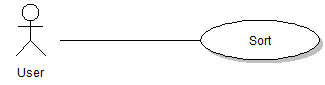
\includegraphics{sort}\\ \hline
Element & Description \\ \hline
Use case name & Sort \\
Goal & User sorts the messages in his inbox. \\
Summary & The user chosoes a value that he wishes the messages to be sorted by. \\
Preconditions &
\begin{enumerate}
\item{}The application is running.
\item{}The user is logged in.
\item{}There are messages to sort.
\end{enumerate} \\ \hline
Flow of Events &
\begin{enumerate}
\item{}The user selects the value he wishes the messages to be sorted by.
\item{}The application sorts the messages and displays them to the user.
\end{enumerate}
\end{tabular}
\caption{Sort textual use case} \label{tab:search}
\end{table}

\begin{table}
\begin{tabular}{p{3cm}p{12cm}}
& 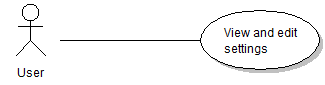
\includegraphics{settings}\\ \hline
Element & Description \\ \hline
Use case name & Settings \\
Goal & The user can alter settings. \\
Summary & The user enters the settings menu and alter the settings to suit his own preferences. \\
Preconditions &
\begin{enumerate}
\item{}The application is running.
\item{}The user is logged in.
\end{enumerate} \\ \hline
Flow of Events &
\begin{enumerate}
\item{}User presses the settings button.
\item{}User alters the settings he wishes to.
\item{}Application saves the alterations.
\end{enumerate}
\end{tabular}
\caption{Settings textual use case} \label{tab:settings}
\end{table}
